
%% bare_conf.tex
%% V1.3
%% 2007/01/11
%% by Michael Shell
%% See:
%% http://www.michaelshell.org/
%% for current contact information.
%%
%% This is a skeleton file demonstrating the use of IEEEtran.cls
%% (requires IEEEtran.cls version 1.7 or later) with an IEEE conference paper.
%%
%% Support sites:
%% http://www.michaelshell.org/tex/ieeetran/
%% http://www.ctan.org/tex-archive/macros/latex/contrib/IEEEtran/
%% and
%% http://www.ieee.org/

%%*************************************************************************
%% Legal Notice:
%% This code is offered as-is without any warranty either expressed or
%% implied; without even the implied warranty of MERCHANTABILITY or
%% FITNESS FOR A PARTICULAR PURPOSE! 
%% User assumes all risk.
%% In no event shall IEEE or any contributor to this code be liable for
%% any damages or losses, including, but not limited to, incidental,
%% consequential, or any other damages, resulting from the use or misuse
%% of any information contained here.
%%
%% All comments are the opinions of their respective authors and are not
%% necessarily endorsed by the IEEE.
%%
%% This work is distributed under the LaTeX Project Public License (LPPL)
%% ( http://www.latex-project.org/ ) version 1.3, and may be freely used,
%% distributed and modified. A copy of the LPPL, version 1.3, is included
%% in the base LaTeX documentation of all distributions of LaTeX released
%% 2003/12/01 or later.
%% Retain all contribution notices and credits.
%% ** Modified files should be clearly indicated as such, including  **
%% ** renaming them and changing author support contact information. **
%%
%% File list of work: IEEEtran.cls, IEEEtran_HOWTO.pdf, bare_adv.tex,
%%                    bare_conf.tex, bare_jrnl.tex, bare_jrnl_compsoc.tex
%%*************************************************************************

% *** Authors should verify (and, if needed, correct) their LaTeX system  ***
% *** with the testflow diagnostic prior to trusting their LaTeX platform ***
% *** with production work. IEEE's font choices can trigger bugs that do  ***
% *** not appear when using other class files.                            ***
% The testflow support page is at:
% http://www.michaelshell.org/tex/testflow/



% Note that the a4paper option is mainly intended so that authors in
% countries using A4 can easily print to A4 and see how their papers will
% look in print - the typesetting of the document will not typically be
% affected with changes in paper size (but the bottom and side margins will).
% Use the testflow package mentioned above to verify correct handling of
% both paper sizes by the user's LaTeX system.
%
% Also note that the "draftcls" or "draftclsnofoot", not "draft", option
% should be used if it is desired that the figures are to be displayed in
% draft mode.
%
\documentclass[conference]{IEEEtran}
% Add the compsoc option for Computer Society conferences.
%
% If IEEEtran.cls has not been installed into the LaTeX system files,
% manually specify the path to it like:
% \documentclass[conference]{../sty/IEEEtran}





% Some very useful LaTeX packages include:
% (uncomment the ones you want to load)


% *** MISC UTILITY PACKAGES ***
%
%\usepackage{ifpdf}
% Heiko Oberdiek's ifpdf.sty is very useful if you need conditional
% compilation based on whether the output is pdf or dvi.
% usage:
% \ifpdf
%   % pdf code
% \else
%   % dvi code
% \fi
% The latest version of ifpdf.sty can be obtained from:
% http://www.ctan.org/tex-archive/macros/latex/contrib/oberdiek/
% Also, note that IEEEtran.cls V1.7 and later provides a builtin
% \ifCLASSINFOpdf conditional that works the same way.
% When switching from latex to pdflatex and vice-versa, the compiler may
% have to be run twice to clear warning/error messages.






% *** CITATION PACKAGES ***
%
\usepackage{cite}
% cite.sty was written by Donald Arseneau
% V1.6 and later of IEEEtran pre-defines the format of the cite.sty package
% \cite{} output to follow that of IEEE. Loading the cite package will
% result in citation numbers being automatically sorted and properly
% "compressed/ranged". e.g., [1], [9], [2], [7], [5], [6] without using
% cite.sty will become [1], [2], [5]--[7], [9] using cite.sty. cite.sty's
% \cite will automatically add leading space, if needed. Use cite.sty's
% noadjust option (cite.sty V3.8 and later) if you want to turn this off.
% cite.sty is already installed on most LaTeX systems. Be sure and use
% version 4.0 (2003-05-27) and later if using hyperref.sty. cite.sty does
% not currently provide for hyperlinked citations.
% The latest version can be obtained at:
% http://www.ctan.org/tex-archive/macros/latex/contrib/cite/
% The documentation is contained in the cite.sty file itself.






% *** GRAPHICS RELATED PACKAGES ***
%
\ifCLASSINFOpdf
  % \usepackage[pdftex]{graphicx}
  \usepackage{graphicx}
  % declare the path(s) where your graphic files are
  % \graphicspath{{../pdf/}{../jpeg/}}
  % and their extensions so you won't have to specify these with
  % every instance of \includegraphics
  % \DeclareGraphicsExtensions{.pdf,.jpeg,.png}
\else
  % or other class option (dvipsone, dvipdf, if not using dvips). graphicx
  % will default to the driver specified in the system graphics.cfg if no
  % driver is specified.
  % \usepackage[dvips]{graphicx}
  % declare the path(s) where your graphic files are
  % \graphicspath{{../eps/}}
  % and their extensions so you won't have to specify these with
  % every instance of \includegraphics
  % \DeclareGraphicsExtensions{.eps}
\fi
% graphicx was written by David Carlisle and Sebastian Rahtz. It is
% required if you want graphics, photos, etc. graphicx.sty is already
% installed on most LaTeX systems. The latest version and documentation can
% be obtained at: 
% http://www.ctan.org/tex-archive/macros/latex/required/graphics/
% Another good source of documentation is "Using Imported Graphics in
% LaTeX2e" by Keith Reckdahl which can be found as epslatex.ps or
% epslatex.pdf at: http://www.ctan.org/tex-archive/info/
%
% latex, and pdflatex in dvi mode, support graphics in encapsulated
% postscript (.eps) format. pdflatex in pdf mode supports graphics
% in .pdf, .jpeg, .png and .mps (metapost) formats. Users should ensure
% that all non-photo figures use a vector format (.eps, .pdf, .mps) and
% not a bitmapped formats (.jpeg, .png). IEEE frowns on bitmapped formats
% which can result in "jaggedy"/blurry rendering of lines and letters as
% well as large increases in file sizes.
%
% You can find documentation about the pdfTeX application at:
% http://www.tug.org/applications/pdftex





% *** MATH PACKAGES ***
%
\usepackage[cmex10]{amsmath}
% A popular package from the American Mathematical Society that provides
% many useful and powerful commands for dealing with mathematics. If using
% it, be sure to load this package with the cmex10 option to ensure that
% only type 1 fonts will utilized at all point sizes. Without this option,
% it is possible that some math symbols, particularly those within
% footnotes, will be rendered in bitmap form which will result in a
% document that can not be IEEE Xplore compliant!
%
% Also, note that the amsmath package sets \interdisplaylinepenalty to 10000
% thus preventing page breaks from occurring within multiline equations. Use:
%\interdisplaylinepenalty=2500
% after loading amsmath to restore such page breaks as IEEEtran.cls normally
% does. amsmath.sty is already installed on most LaTeX systems. The latest
% version and documentation can be obtained at:
% http://www.ctan.org/tex-archive/macros/latex/required/amslatex/math/





% *** SPECIALIZED LIST PACKAGES ***
%
%\usepackage{algorithmic}
% algorithmic.sty was written by Peter Williams and Rogerio Brito.
% This package provides an algorithmic environment fo describing algorithms.
% You can use the algorithmic environment in-text or within a figure
% environment to provide for a floating algorithm. Do NOT use the algorithm
% floating environment provided by algorithm.sty (by the same authors) or
% algorithm2e.sty (by Christophe Fiorio) as IEEE does not use dedicated
% algorithm float types and packages that provide these will not provide
% correct IEEE style captions. The latest version and documentation of
% algorithmic.sty can be obtained at:
% http://www.ctan.org/tex-archive/macros/latex/contrib/algorithms/
% There is also a support site at:
% http://algorithms.berlios.de/index.html
% Also of interest may be the (relatively newer and more customizable)
% algorithmicx.sty package by Szasz Janos:
% http://www.ctan.org/tex-archive/macros/latex/contrib/algorithmicx/




% *** ALIGNMENT PACKAGES ***
%
\usepackage{array}
% Frank Mittelbach's and David Carlisle's array.sty patches and improves
% the standard LaTeX2e array and tabular environments to provide better
% appearance and additional user controls. As the default LaTeX2e table
% generation code is lacking to the point of almost being broken with
% respect to the quality of the end results, all users are strongly
% advised to use an enhanced (at the very least that provided by array.sty)
% set of table tools. array.sty is already installed on most systems. The
% latest version and documentation can be obtained at:
% http://www.ctan.org/tex-archive/macros/latex/required/tools/


%\usepackage{mdwmath}
%\usepackage{mdwtab}
% Also highly recommended is Mark Wooding's extremely powerful MDW tools,
% especially mdwmath.sty and mdwtab.sty which are used to format equations
% and tables, respectively. The MDWtools set is already installed on most
% LaTeX systems. The lastest version and documentation is available at:
% http://www.ctan.org/tex-archive/macros/latex/contrib/mdwtools/


% IEEEtran contains the IEEEeqnarray family of commands that can be used to
% generate multiline equations as well as matrices, tables, etc., of high
% quality.


%\usepackage{eqparbox}
% Also of notable interest is Scott Pakin's eqparbox package for creating
% (automatically sized) equal width boxes - aka "natural width parboxes".
% Available at:
% http://www.ctan.org/tex-archive/macros/latex/contrib/eqparbox/




% *** SUBFIGURE PACKAGES ***
%\usepackage[tight,footnotesize]{subfigure}
% subfigure.sty was written by Steven Douglas Cochran. This package makes it
% easy to put subfigures in your figures. e.g., "Figure 1a and 1b". For IEEE
% work, it is a good idea to load it with the tight package option to reduce
% the amount of white space around the subfigures. subfigure.sty is already
% installed on most LaTeX systems. The latest version and documentation can
% be obtained at:
% http://www.ctan.org/tex-archive/obsolete/macros/latex/contrib/subfigure/
% subfigure.sty has been superceeded by subfig.sty.



%\usepackage[caption=false]{caption}
%\usepackage[font=footnotesize]{subfig}
% subfig.sty, also written by Steven Douglas Cochran, is the modern
% replacement for subfigure.sty. However, subfig.sty requires and
% automatically loads Axel Sommerfeldt's caption.sty which will override
% IEEEtran.cls handling of captions and this will result in nonIEEE style
% figure/table captions. To prevent this problem, be sure and preload
% caption.sty with its "caption=false" package option. This is will preserve
% IEEEtran.cls handing of captions. Version 1.3 (2005/06/28) and later 
% (recommended due to many improvements over 1.2) of subfig.sty supports
% the caption=false option directly:
%\usepackage[caption=false,font=footnotesize]{subfig}
%
% The latest version and documentation can be obtained at:
% http://www.ctan.org/tex-archive/macros/latex/contrib/subfig/
% The latest version and documentation of caption.sty can be obtained at:
% http://www.ctan.org/tex-archive/macros/latex/contrib/caption/




% *** FLOAT PACKAGES ***
%
%\usepackage{fixltx2e}
% fixltx2e, the successor to the earlier fix2col.sty, was written by
% Frank Mittelbach and David Carlisle. This package corrects a few problems
% in the LaTeX2e kernel, the most notable of which is that in current
% LaTeX2e releases, the ordering of single and double column floats is not
% guaranteed to be preserved. Thus, an unpatched LaTeX2e can allow a
% single column figure to be placed prior to an earlier double column
% figure. The latest version and documentation can be found at:
% http://www.ctan.org/tex-archive/macros/latex/base/



\usepackage{stfloats}
% stfloats.sty was written by Sigitas Tolusis. This package gives LaTeX2e
% the ability to do double column floats at the bottom of the page as well
% as the top. (e.g., "\begin{figure*}[!b]" is not normally possible in
% LaTeX2e). It also provides a command:
%\fnbelowfloat
% to enable the placement of footnotes below bottom floats (the standard
% LaTeX2e kernel puts them above bottom floats). This is an invasive package
% which rewrites many portions of the LaTeX2e float routines. It may not work
% with other packages that modify the LaTeX2e float routines. The latest
% version and documentation can be obtained at:
% http://www.ctan.org/tex-archive/macros/latex/contrib/sttools/
% Documentation is contained in the stfloats.sty comments as well as in the
% presfull.pdf file. Do not use the stfloats baselinefloat ability as IEEE
% does not allow \baselineskip to stretch. Authors submitting work to the
% IEEE should note that IEEE rarely uses double column equations and
% that authors should try to avoid such use. Do not be tempted to use the
% cuted.sty or midfloat.sty packages (also by Sigitas Tolusis) as IEEE does
% not format its papers in such ways.





% *** PDF, URL AND HYPERLINK PACKAGES ***
%
%\usepackage{url}
% url.sty was written by Donald Arseneau. It provides better support for
% handling and breaking URLs. url.sty is already installed on most LaTeX
% systems. The latest version can be obtained at:
% http://www.ctan.org/tex-archive/macros/latex/contrib/misc/
% Read the url.sty source comments for usage information. Basically,
% \url{my_url_here}.





% *** Do not adjust lengths that control margins, column widths, etc. ***
% *** Do not use packages that alter fonts (such as pslatex).         ***
% There should be no need to do such things with IEEEtran.cls V1.6 and later.
% (Unless specifically asked to do so by the journal or conference you plan
% to submit to, of course. )


% correct bad hyphenation here
% \hyphenation{op-tical net-works semi-conduc-tor}

\usepackage{multirow}
\usepackage{paralist}
\usepackage[font=normalsize]{caption}
\usepackage{color}

\newcommand{\red}[1]{\colorbox{red}{#1}}

\begin{document}
%
% paper title
% can use linebreaks \\ within to get better formatting as desired
\title{Integration and Automation of\\ Data Preparation and Data Mining}


% author names and affiliations
% use a multiple column layout for up to three different
% affiliations

% \author{\IEEEauthorblockN{Shrikanth Narayanan}
\IEEEauthorblockA{Spatial Sciences Institute \\ Department of Computer Science \\ University of Southern California \\ Email: nara471@usc.edu}
 \and
\IEEEauthorblockN{Ayush Jaiswal}
\IEEEauthorblockA{Department of Computer Science \\ University of Southern California \\ Email: ajaiswal@usc.edu}
  \and
\IEEEauthorblockN{Yao-Yi Chiang}
 \IEEEauthorblockA{Spatial Sciences Institute \\ University of Southern California \\ Email: yaoyic@usc.edu}
  \and
\IEEEauthorblockN{Yanhui Geng}
 \IEEEauthorblockA{Huawei Technologies \\ Email: geng.yanhui@huawei.com}
  \and
\IEEEauthorblockN{Craig A. Knoblock}
 \IEEEauthorblockA{Information Sciences Institute \\ Department of Computer Science \\ University of Southern California \\ Email: knoblock@isi.edu}
  \and
\IEEEauthorblockN{Pedro Szekely}
 \IEEEauthorblockA{Information Sciences Institute \\ Department of Computer Science \\ University of Southern California \\ Email: pszekely@isi.edu}
}
\author{\IEEEauthorblockN{}
\IEEEauthorblockA{ \\  \\ \\ }
 \and
\IEEEauthorblockN{\\}
\IEEEauthorblockA{ \\  \\ \\}
  \and
\IEEEauthorblockN{\\}
 \IEEEauthorblockA{\\ \\}
  \and
\IEEEauthorblockN{\\}
 \IEEEauthorblockA{\\}
  \and
\IEEEauthorblockN{\\}
 \IEEEauthorblockA{\\ \\ \\ \\}
  \and
\IEEEauthorblockN{\\}
 \IEEEauthorblockA{\\ \\ \\ \\}
}

% conference papers do not typically use \thanks and this command
% is locked out in conference mode. If really needed, such as for
% the acknowledgment of grants, issue a \IEEEoverridecommandlockouts
% after \documentclass

% for over three affiliations, or if they all won't fit within the width
% of the page, use this alternative format:
% 
%\author{\IEEEauthorblockN{Michael Shell\IEEEauthorrefmark{1},
%Homer Simpson\IEEEauthorrefmark{2},
%James Kirk\IEEEauthorrefmark{3}, 
%Montgomery Scott\IEEEauthorrefmark{3} and
%Eldon Tyrell\IEEEauthorrefmark{4}}
%\IEEEauthorblockA{\IEEEauthorrefmark{1}School of Electrical and Computer Engineering\\
%Georgia Institute of Technology,
%Atlanta, Georgia 30332--0250\\ Email: see http://www.michaelshell.org/contact.html}
%\IEEEauthorblockA{\IEEEauthorrefmark{2}Twentieth Century Fox, Springfield, USA\\
%Email: homer@thesimpsons.com}
%\IEEEauthorblockA{\IEEEauthorrefmark{3}Starfleet Academy, San Francisco, California 96678-2391\\
%Telephone: (800) 555--1212, Fax: (888) 555--1212}
%\IEEEauthorblockA{\IEEEauthorrefmark{4}Tyrell Inc., 123 Replicant Street, Los Angeles, California 90210--4321}}




% use for special paper notices
%\IEEEspecialpapernotice{(Invited Paper)}




% make the title area
\maketitle

\begin{abstract}
Data mining tasks typically require significant effort in data preparation to find, transform, integrate and prepare the data for the relevant data mining tools.  In addition, the work performed in data preparation is often not recorded and is difficult to reproduce from the raw data.  In this paper we present an integrated approach to data preparation and data mining that combines the two steps into a single integrated process and maintains detailed metadata about the data sources, the steps in the process, and the resulting learned classifier produced from data mining algorithms.  We present results on an example scenario, which shows that our approach provides significant reduction in the time in takes to perform a data mining task. 
\end{abstract}

% IEEEtran.cls defaults to using nonbold math in the Abstract.
% This preserves the distinction between vectors and scalars. However,
% if the conference you are submitting to favors bold math in the abstract,
% then you can use LaTeX's standard command \boldmath at the very start
% of the abstract to achieve this. Many IEEE journals/conferences frown on
% math in the abstract anyway.

% no keywords




% For peer review papers, you can put extra information on the cover
% page as needed:
% \ifCLASSOPTIONpeerreview
% \begin{center} \bfseries EDICS Category: 3-BBND \end{center}
% \fi
%
% For peerreview papers, this IEEEtran command inserts a page break and
% creates the second title. It will be ignored for other modes.
\IEEEpeerreviewmaketitle

\section{Introduction}
%Most of the work is still in preparing the data
%Data preparation is done manually - either by writing a program or using data manipulation software (Excel)
While the quality and ease of use of data mining libraries such as in R~\cite{R2008} and Weka~\cite{Hall2009} is excellent, users must spend significant effort to prepare raw data for use in these libraries. In practice, the data preparation task is separate from the data mining process and very often requires data source dependent and repetitive manual work, such as applying Structured Query Language (SQL) statements to extract and aggregate database records, using Microsoft Excel to clean and normalize datasets of structured text files, and writing scripts to apply complex transformations (e.g., in Python). This practice does not scale when the data size becomes larger and the number of data sources increases.

In a previous work, Knoblock et al.~\cite{knoblock11:lisc,knoblock12:eswc} developed an interactive approach to extracting, modeling, and publishing data in a system called Karma.\footnote{See http://www.isi.edu/integration/karma for a video demonstration and details on Karma. The software is available as open source (Apache 2 License).} Karma allows an end-user to solve their own integration tasks without having to program those tasks. Karma can semi-automatically build a semantic description (a model) of a data source. This semantic description makes it possible to rapidly convert a set of sources (represented in Extensible Markup Language (XML), Javascript Object Notation (JSON), structured text files, or databases) into a shared domain model, which supports the integrated reasoning and processing of data across many sources. Once a user models the data sources, Karma can automatically converts the raw data into any of a variety of formats.

In this paper we present an integrated approach built on Karma for information integration and data mining. Our approach combines the steps in data preparation and data mining into a single integrated process and maintains detailed metadata about the data sources. We show that a user can use our approach to rapidly clean, normalize, restructure, integrate data collected from multiple mobile sensors, and then apply machine learning algorithms from a library of algorithms to perform a data mining task. We demonstrate these capabilities using a data mining task of predicting the mode of transport of a user given the sensor data collected via his/her cellphone. The challenge here is how to perform a data mining task, such that there is an sizable reduction in overall user time and effort in preparing the data set from its raw form and invoking the prediction service. We compare our approach with a baseline approach that uses Microsoft Excel for most of the data preparation tasks. We show how Karma supports the required steps for data preparation and data mining, and yields a significant reduction in time and effort.

The remainder of this paper is organized as follows. Section~2 describes a motivating data mining problem on prediction of mode of transport from mobile sensor data. Section~3 presents our integrated approach to data preparation and data mining. Section~4 describes the steps of using Excel to prepare raw data for data mining. Section~5 reports on our experimental results. Section~6 discusses the related work, and Section~7 presents discussion and future work.

\begin{figure}[ht!]
\centering
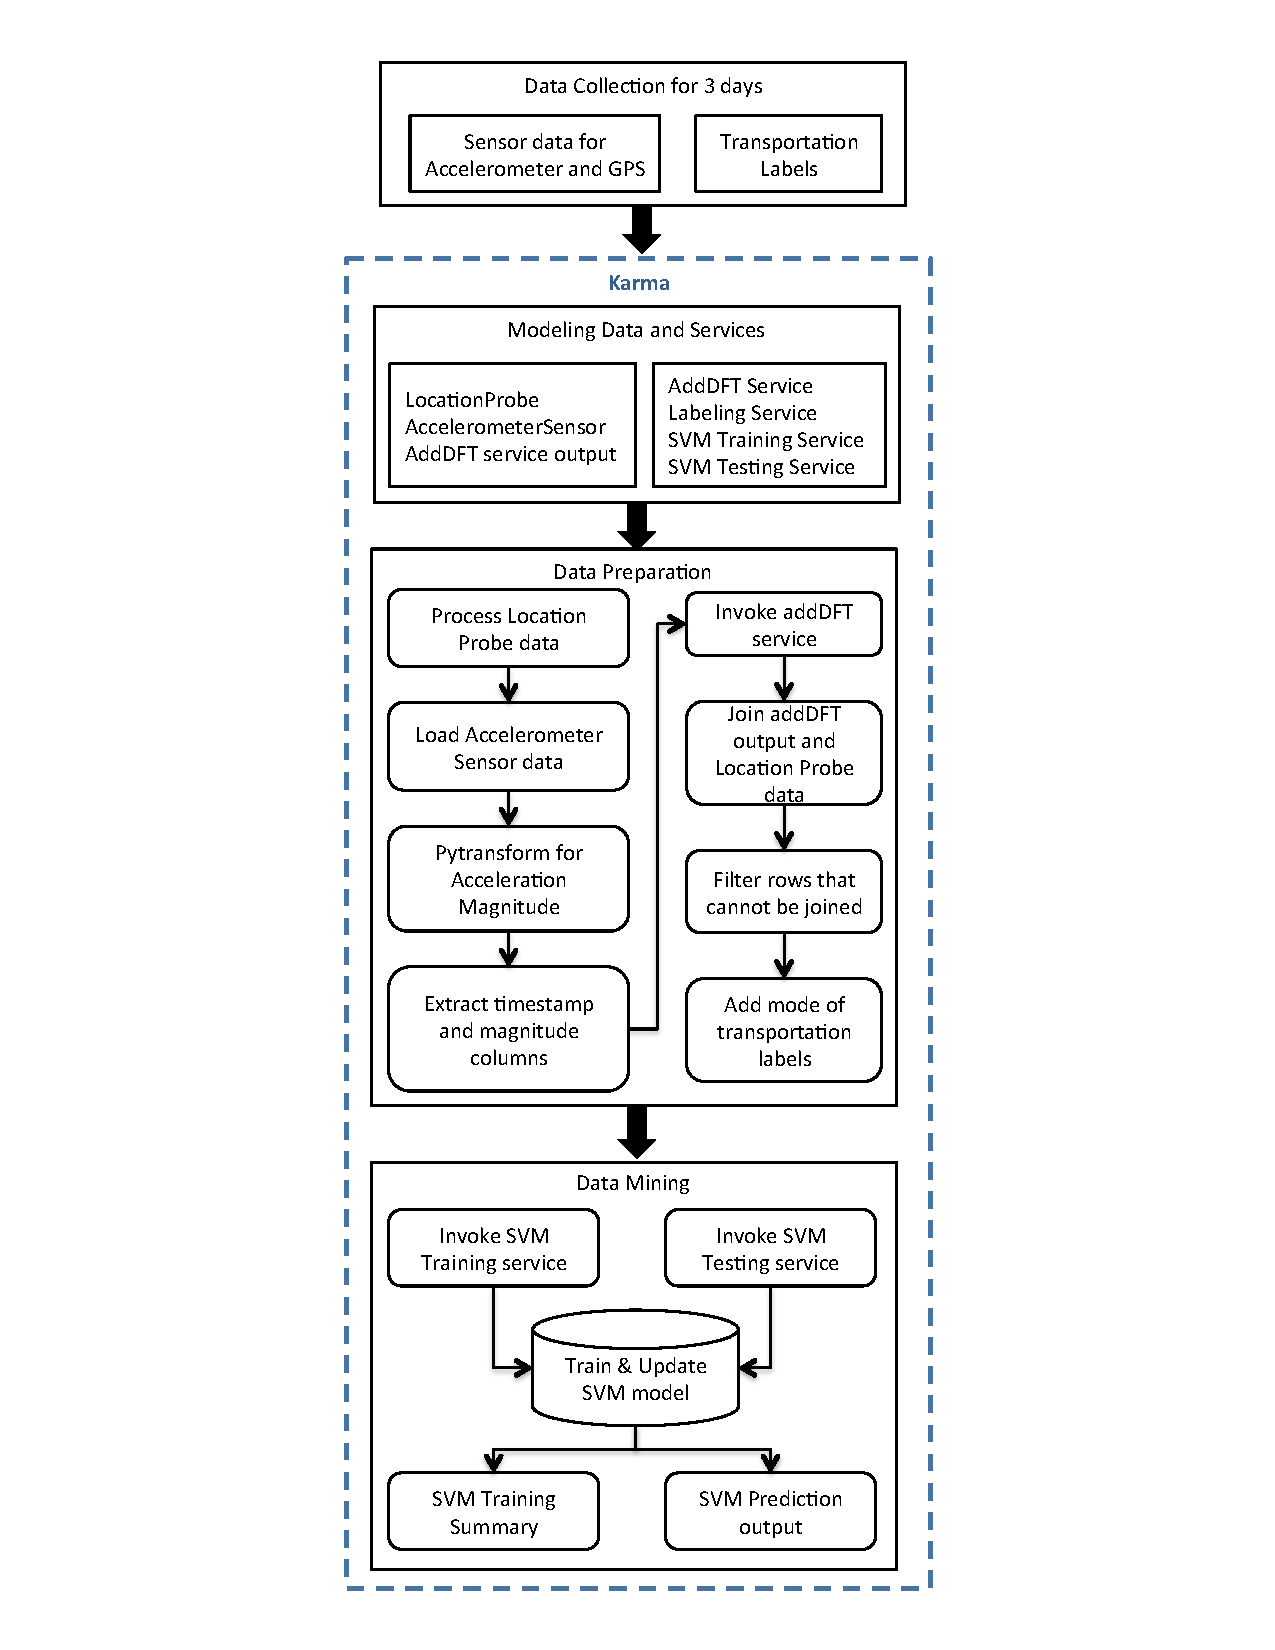
\includegraphics[width=80mm]{img/system_diagram.pdf}
\caption{System block diagram\label{fig:system_diagram}}
\end{figure}

% An example of a floating figure using the graphicx package.
% Note that \label must occur AFTER (or within) \caption.
% For figures, \caption should occur after the \includegraphics.
% Note that IEEEtran v1.7 and later has special internal code that
% is designed to preserve the operation of \label within \caption
% even when the captionsoff option is in effect. However, because
% of issues like this, it may be the safest practice to put all your
% \label just after \caption rather than within \caption{}.
%
% Reminder: the "draftcls" or "draftclsnofoot", not "draft", class
% option should be used if it is desired that the figures are to be
% displayed while in draft mode.
%
%\begin{figure}[!t]
%\centering
%\includegraphics[width=2.5in]{myfigure}
% where an .eps filename suffix will be assumed under latex, 
% and a .pdf suffix will be assumed for pdflatex; or what has been declared
% via \DeclareGraphicsExtensions.
%\caption{Simulation Results}
%\label{fig_sim}
%\end{figure}

% Note that IEEE typically puts floats only at the top, even when this
% results in a large percentage of a column being occupied by floats.


% An example of a double column floating figure using two subfigures.
% (The subfig.sty package must be loaded for this to work.)
% The subfigure \label commands are set within each subfloat command, the
% \label for the overall figure must come after \caption.
% \hfil must be used as a separator to get equal spacing.
% The subfigure.sty package works much the same way, except \subfigure is
% used instead of \subfloat.
%
%\begin{figure*}[!t]
%\centerline{\subfloat[Case I]\includegraphics[width=2.5in]{subfigcase1}%
%\label{fig_first_case}}
%\hfil
%\subfloat[Case II]{\includegraphics[width=2.5in]{subfigcase2}%
%\label{fig_second_case}}}
%\caption{Simulation results}
%\label{fig_sim}
%\end{figure*}
%
% Note that often IEEE papers with subfigures do not employ subfigure
% captions (using the optional argument to \subfloat), but instead will
% reference/describe all of them (a), (b), etc., within the main caption.


% An example of a floating table. Note that, for IEEE style tables, the 
% \caption command should come BEFORE the table. Table text will default to
% \footnotesize as IEEE normally uses this smaller font for tables.
% The \label must come after \caption as always.
%
%\begin{table}[!t]
%% increase table row spacing, adjust to taste
%\renewcommand{\arraystretch}{1.3}
% if using array.sty, it might be a good idea to tweak the value of
% \extrarowheight as needed to properly center the text within the cells
%\caption{An Example of a Table}
%\label{table_example}
%\centering
%% Some packages, such as MDW tools, offer better commands for making tables
%% than the plain LaTeX2e tabular which is used here.
%\begin{tabular}{|c||c|}
%\hline
%One & Two\\
%\hline
%Three & Four\\
%\hline
%\end{tabular}
%\end{table}


% Note that IEEE does not put floats in the very first column - or typically
% anywhere on the first page for that matter. Also, in-text middle ("here")
% positioning is not used. Most IEEE journals/conferences use top floats
% exclusively. Note that, LaTeX2e, unlike IEEE journals/conferences, places
% footnotes above bottom floats. This can be corrected via the \fnbelowfloat
% command of the stfloats package.

\section{Motivating Problem}

As an example of a data mining task, we consider the problem of predicting the mode of transport of a mobile user. Mode of transport prediction is an interesting problem in data mining. It helps in providing contextual information about the user that can be used in building intelligent smartphone applications.

Reddy et al. [5] describe a method for predicting the mode of transport of a mobile user by applying the Decision Trees algorithm with features as the Discrete Fourier Transform (DFT) energy coefficients at 1Hz, 2Hz, and 3Hz of acceleration magnitude, the accelerometer variance, and the speed recorded by the GPS sensor. The features are derived from data collected from the accelerometer and the GPS sensors on a mobile device. Our method of predicting the mode of transport is similar to theirs as we use the Support Vector Machine (SVM) algorithm with similar features. We use GPS accuracy as a feature instead of accelerometer variance, keeping the rest of the features the same.

To acquire training and testing data, we use an application that collects accelerometer and GPS readings on mobile phones. We asked users to record their mode of transportation while using the application in order to acquire the data to build the prediction model. The data mining system derives the aforementioned features from the sensor data and merges the mode of transport labels noted by the user with the features, as classes, for mining.

The collected data is hardly ever ready to use directly in real life scenarios. We have to prepare it for mining through multiple transformation steps, such as dealing with missing values, discretization, and normalization. Moreover, even if the data is in tabular form, in many cases, we cannot use the columns as features for data mining libraries directly. We have to compute useful features by using values in multiple columns. In the example case of mode of transport prediction, we calculate acceleration magnitude from the acceleration recorded by the accelerometer along the X, Y, and Z dimensions. We then calculate DFT energy coefficients at 1Hz, 2Hz, and 3Hz of the acceleration magnitude for every 1 second time window. We then discretize the data, which contains multiple entries every second, to the nearest second. 

Many data mining tasks use data from multiple sources that have to be merged in order to derive features from them, such as those performed by large organizations on data collected from different branches and departments within them. The data used by the algorithm that we employ in our example case is derived from three sources, i.e., the accelerometer sensor, the GPS sensor, and the user’s mode of transportation notes. We merge the data by making use of timestamps contained in all the three sources.

In general, after the data is prepared, machine learning algorithms are applied to it to train the prediction model and to test it, or to perform cross-validation. In our case, we train a prediction model using the SVM algorithm and test it. The final set of features consists of DFT energy coefficients at 1Hz, 2Hz, and 3Hz, speed recorded by the GPS sensor, and GPS accuracy.

These parts of the entire data mining system motivate the development of a complete end-to-end system that offers complex data transformations (as in-built features, extensions, or services), data merging capabilities, invocation of various machine learning algorithms for application and comparison, and display of results in a meaningful manner.
\section{Approach}

In general, a data mining task will have the following steps - data collection, data integration and cleaning, transformation and selection, data mining and evaluation \cite{Fayyad:1996:DMK:257938.257942}. It has been estimated that data preparation - integration, cleaning, selection and transformation, accounts for a significant portion of the time spent on a data mining project. In our approach to demonstrate the end-to-end process of data preparation and data mining, we select the task of predicting the mode of transport for a user, given the sensor data collected by the mobile phones. Our approach enables users to integrate data from a variety of sources without exposing them to the underlying complexity of data integration and exchange. Figure \ref{fig:system_diagram} shows the different blocks of system.
 
\subsection{Data Collection}
We collect the mobile sensor data using a custom Android application built using the funf\footnote{http://inabox.funf.org} sensing framework. The application records the readings from the Accelerometer and the Global Positioning System (GPS) sensors, archives and uploads the collected data to a Dropbox\footnote{http://dropbox.com} account every 24 hours. Our users collected data for three days, yielding datasets consisting of Comma Separated Value (CSV) files. Each dataset is comprised of 3 files:

\begin{enumerate}
  \item \textit{LocationProbe.csv}: Contains positioning data from the GPS sensors and has 47 columns describing the user's location, speed, bearing, etc.
  \item \textit{AccelerometerSensor.csv}: Contains coordinate values from the accelerometers
  \item \textit{TransportationLabels.csv}: The user collecting the data has to label each mode of transport that they use and the specific intervals of the day when they use it
\end{enumerate} 

\begin{figure}[h]
\centering
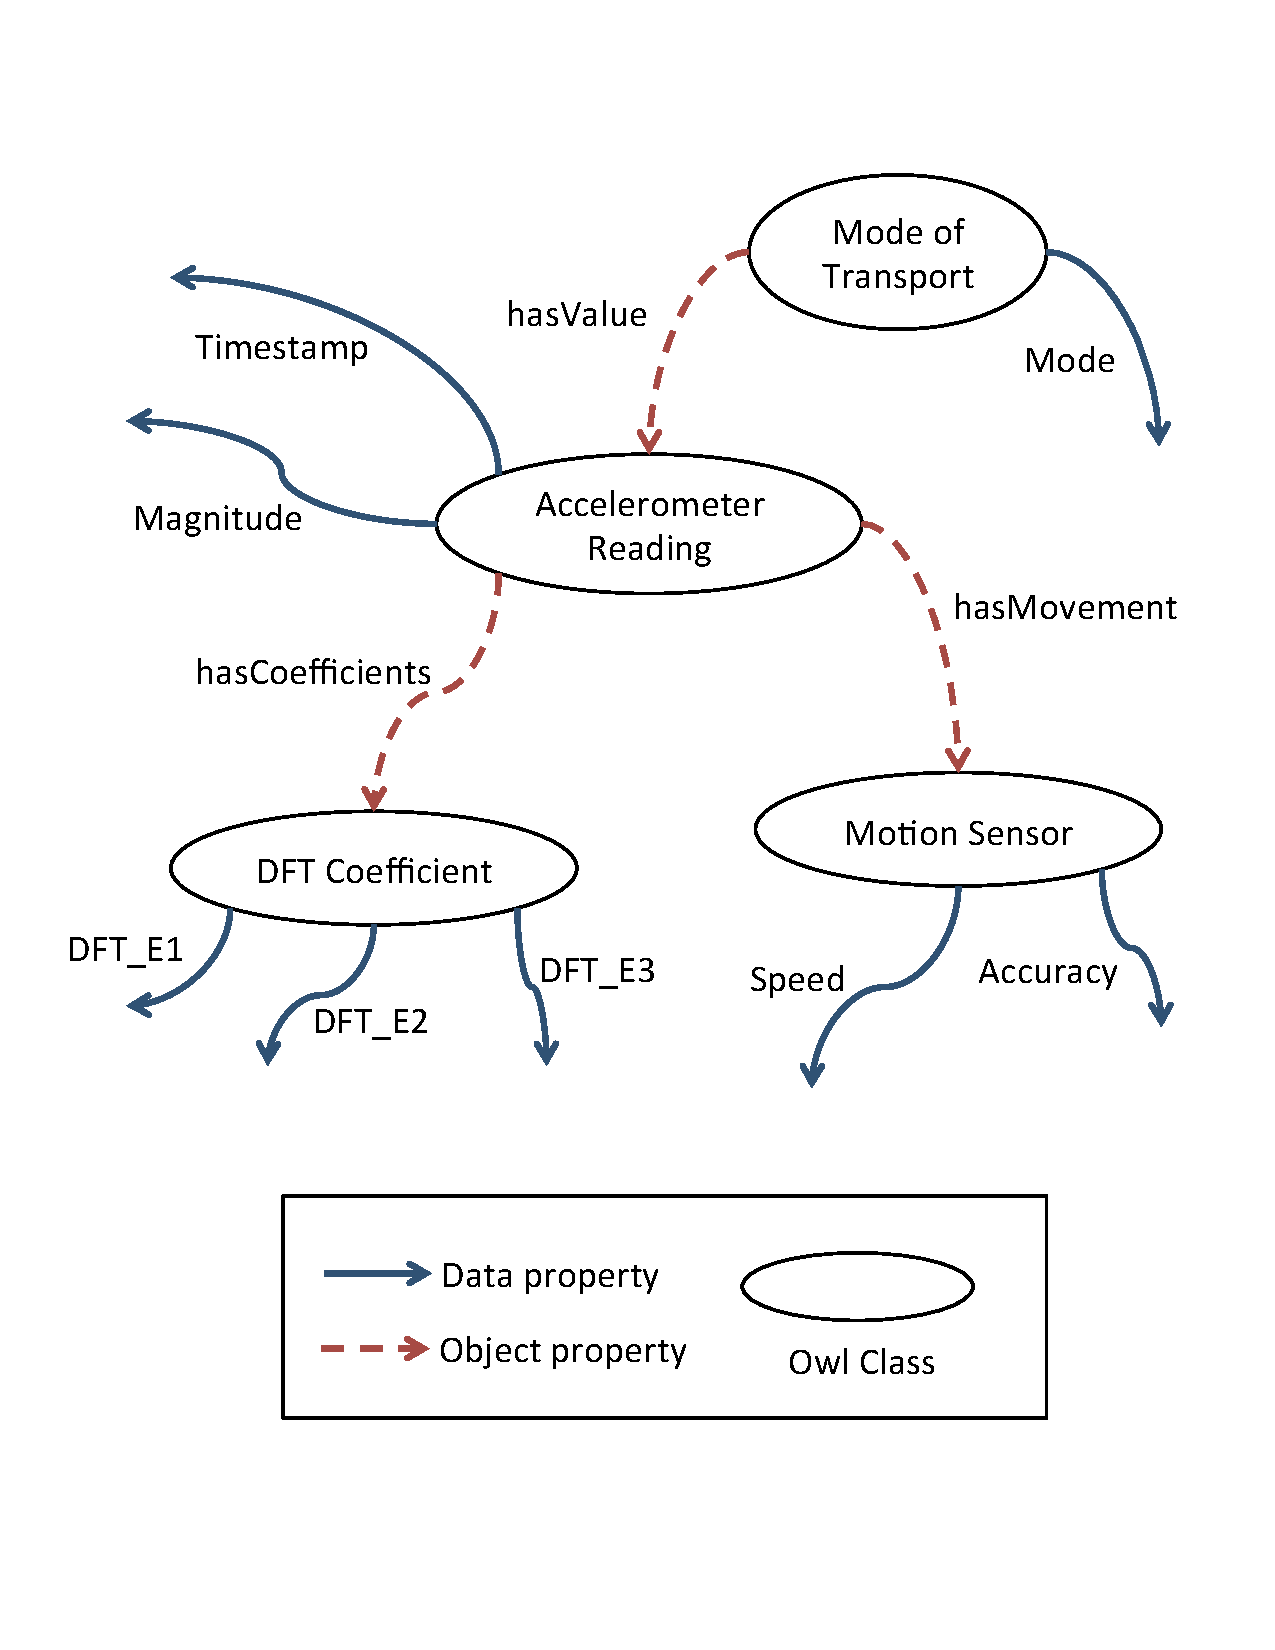
\includegraphics[width=90mm]{img/ontology.pdf}
\caption{Ontology used in for the mode of transportation data\label{fig:ontology}}
\end{figure}

\subsection{Processing with Karma}
The steps using Karma are divided into two parts:
\begin{enumerate}
  \item \textbf{Karma setup}: These are tasks that are performed only the first time. They include modeling the three web services, addDFT, getLabel, and svmTraining, which are explained later, as well as modeling the two raw datasets AccelerometerSensor and LocationProbe. All transformations and processing done here is recorded by Karma and can be played automatically for the other datasets. 
  \item \textbf{Karma execution}: The Karma execution tasks are ones that are repeated for each datasets. They mainly include tasks such as service invocation, joining datasets, and publishing data in the Resource Description Framework (RDF).
\end{enumerate} 

\begin{figure}[bp]
\centering
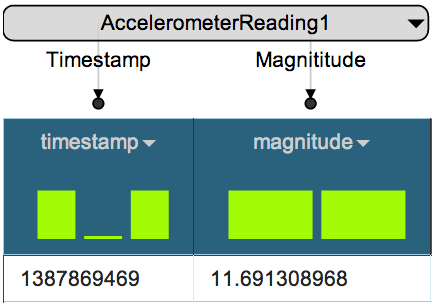
\includegraphics[width=55mm]{img/DFTservice}
\caption{Semantic model for addDFT service\label{fig:dftService}}
\end{figure}

\subsubsection{Karma Setup} 
The work on Karma\cite{knoblock12:eswc} shows how to map structured data to RDF using an ontology. Karma uses a two step process to map data to ontology. The mapping of columns to semantic types and specifying relationships between the semantic types is demonstrated in the work on the Smithsonian dataset\cite{szekely14:ijhac}. When we map our services to our ontology, we attach additional properties to the model along with the semantic type mappings that enables Karma to mark them as a service model. A service model is used to invoke a web service using the columns mapped as inputs to the service. We create an ontology for the mode of transportation data and use it to model our services and data sources. We do not add the ontology creation time in the setup time because such ontologies address a larger domain model and evolve over a period of time. Hence we assume that the ontology was created beforehand. We discuss our ontology and modeling of the services and data sources in the remaining part of the section.

\begin{figure*}[ht!]
\centering
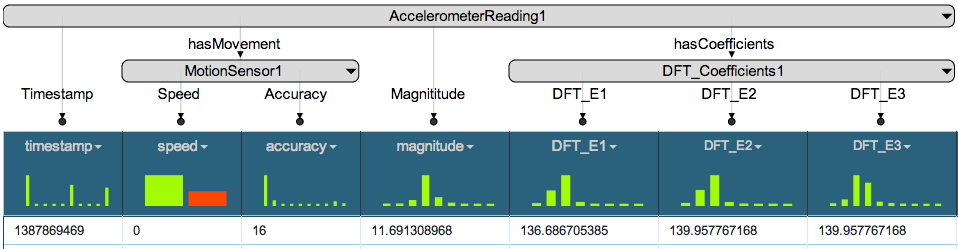
\includegraphics[width=180mm]{img/getLabelService}
\caption{Semantic model for getLabel service\label{fig:imgGetLabelService}}
\end{figure*}

\begin{figure*}[bp]
\centering
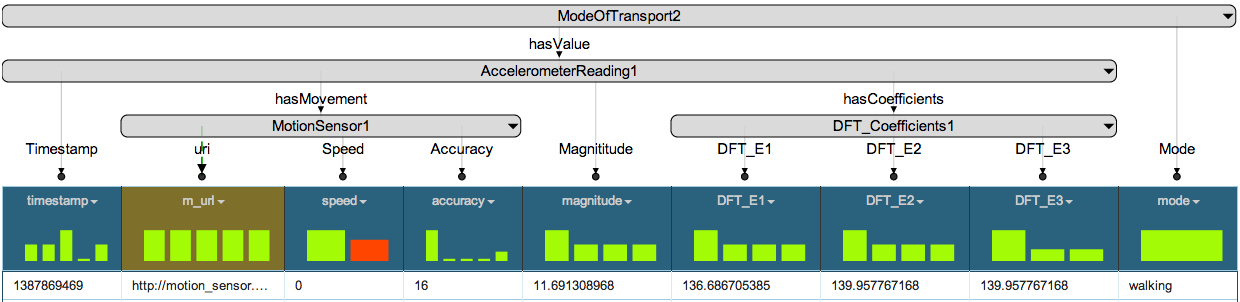
\includegraphics[width=180mm]{img/svmService}
\caption{Semantic model of SVM --- training and testing services\label{fig:svmService}}
\end{figure*}

Figure \ref{fig:ontology} shows the mode of transportation ontology. It contains 4 classes:
\begin{enumerate}
  \item \textit{ModeOfTransport}: Contains a data property for the mode of transportation label
  \item \textit{AccelerometerReading}: Contains data properties for timestamp and acceleration magnitude. The object property --- `hasMovement' connects it to MotionSensor. Similarity, `hasCoefficient' object property connects the AccelerometerReading class to DFT\_Coefficient
  \item \textit{MotionSensor}: Contains data properties for speed and accuracy components of the location probe data
  \item \textit{DFT\_Coefficient}: Contains data properties for the DFT energy coefficients at 1Hz, 2Hz and 3Hz
\end{enumerate} 

We will model three services that we require in our prediction task. Figures \ref{fig:dftService}, \ref{fig:imgGetLabelService} and \ref{fig:svmService} show the models for these services.

The `addDFT' service is a Hypertext Transfer Protocol (HTTP) POST service that calculates the DFT energy coefficients for acceleration magnitude at 1Hz, 2Hz and 3Hz. The input to this service is a CSV file that contains two columns --- timestamp and acceleration magnitude. The DFT values are calculated over a time window of one second. The output generated is a CSV file having the columns --- timestamp, magnitude and the DFT energy coefficients. To model this service, we map the timestamp and magnitude column of our sample CSV file to the appropriate classes. As shown in Figure \ref{fig:dftService}, we set the semantic type of the timestamp column to `timestamp', which is a property of the `AccelerometerReading' class. We then map the magnitude column using the `Magnitude' property of the `AccelerometerReading' class. We set the service URL for the addDFT service and publish the model.

The `getLabel' service is a HTTP POST service that adds the mode of transportation label provided by the user for each row in the input file, using the timestamp values. The output produced is a CSV file containing all the columns of the input with an additional column for labels. To model this service, we map all the columns of our sample CSV file to the appropriate classes excluding the mode column. Figure \ref{fig:imgGetLabelService} shows the column mappings and relationships between the classes, displayed on the Karma interface. We map the speed and accuracy columns to the MotionSensor class using the respective data properties. The timestamp and magnitude are mapped to the AccelerometerReading class. After setting all the semantic types, we set the service URL and other options that are required while invoking the service and publish the model. 

The SVM service has two parts --- training and testing. Both  services take the same set of inputs and have identical semantic types for their corresponding columns. Figure \ref{fig:svmService} shows the semantic model for the SVM training and testing services. The model is very similar to the getLabel service shown in  Figure \ref{fig:imgGetLabelService}. For the SVM service, we map the `mode' column that contains the mode of transportation labels to the `ModeOfTransport' class. The rest of the mappings are discussed in the previous paragraph. We use different service URLs when we publish the SVM training and testing service models. These services also differ in the output that they produce. The training service returns a summary of the SVM model that was trained. In order to distinguish our prediction models, we specify a unique tag in the URL when we train the model. This tag serves as an identifier when we test the model. The testing service produces the prediction output along with the confusion matrix. The output for both the training and testing service is in JSON format. They both consume CSV data in the POST payload.

\begin{figure*}[ht!]
\centering
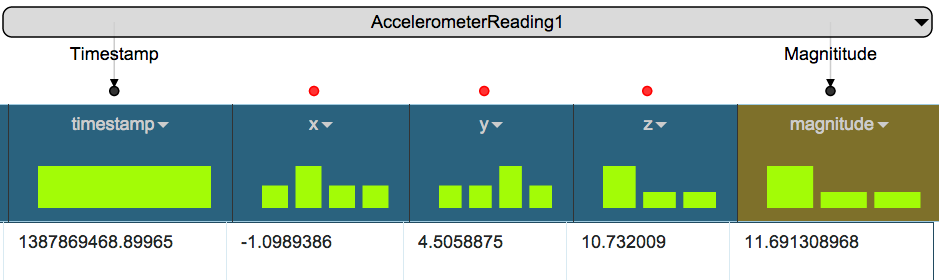
\includegraphics[width=117mm]{img/AccelerometerReadingModel}
\caption{Semantic model for the AccelerometerSensor dataset.\label{fig:AccelerometerReadingModel}}
\end{figure*}

\begin{figure*}[b]
\centering
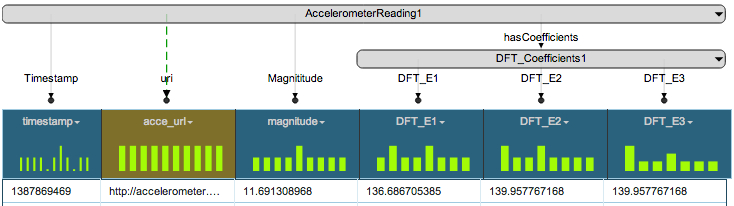
\includegraphics[width=177mm]{img/DFToutput}
\caption{Semantic model of the output generated by addDFT service. \label{fig:DFToutput}}
\end{figure*}

After modeling the services, we model our data sources because the raw data needs to be cleaned and transformed before it can be fed to our services. Karma records the transformations that we perform while modeling the data and replays it when we apply the model on a new file from our data set. After modeling the data, we publish the resulting RDF. Figures \ref{fig:AccelerometerReadingModel}, \ref{fig:DFToutput}, and \ref{fig:motionSensorModel} show the models for our data sources.

Starting with the AccelerometerSensor file, we add the magnitude column using a Python transformation, which is available as a feature in Karma. In this transformation, we calculate the magnitude values using acceleration along x, y, and z coordinates available in the raw data, and by using standard library functions in Python. Figure \ref{fig:AccelerometerReadingModel} shows the resulting model in Karma. The magnitude column appears in yellow color because it is added using a Python transformation and indicates that it is not a part of the original file that is uploaded in Karma. After mapping the semantic types and generating URLs for the classes, we publish the model.

The next data source we model is the output of the addDFT service which is shown in Figure \ref{fig:DFToutput}. The output is a CSV file with the columns --- timestamp, magnitude and DFT energy coefficient values at 1Hz, 2Hz and 3Hz. The addDFT service appends three columns to the input file having headers --- `DFT\_E1', `DFT\_E2' and `DFT\_E3', as shown in Figure \ref{fig:DFToutput}. We map the three columns containing the DFT energy coefficients to the `DFT\_Coefficient' class. The timestamp and magnitude columns are mapped to the `AccelerometerReading' class. We add an additional column, `acce\_url', using a Python transformation and populate it by appending the timestamp values to a base Uniform Resource Identifier (URI). The `acce\_url' column is mapped as the URI for the `AccelerometerReading' class. It is not necessary to have URIs for every class in the model. We add the URI for `AccelerometerReading' class because it is required by Karma to perform join operations.

\begin{figure*}[ht!]
\centering
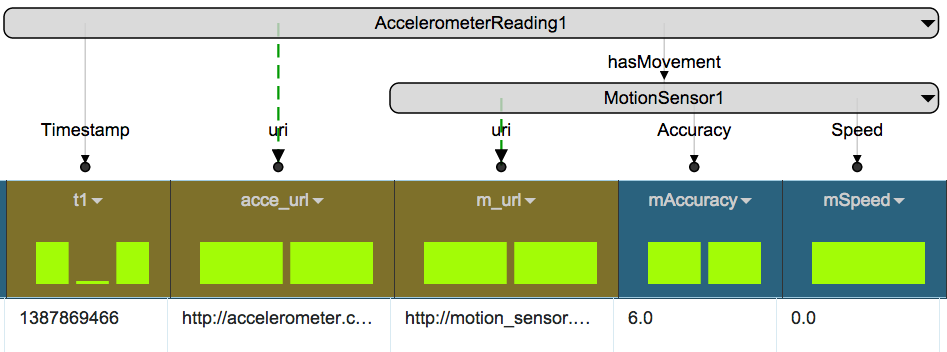
\includegraphics[width=130mm]{img/motionSensorModel}
\caption{Semantic model for the Location probe dataset}
\label{fig:motionSensorModel}
\end{figure*}

The LocationProbe file contains 47 columns, some of them are --- \textit{id, device, timestamp, mAccuracy, mAltitude, mBearing, mElapsedRealtimeNanos, mExtras\_networkLocationSource, mExtras\_networkLocationType, mExtras\_travelState, mHasAccuracy, mHasAltitude, mHasBearing, mHasSpeed, mLatitude, mLongitude, mProvider, mSpeed, mTime, timestamp, etc}. Out of these we only use `timestamp', `mSpeed' and `mAccuracy'. To model this data source, we hide all the unwanted columns after loading the CSV file. As shown in Figure \ref{fig:motionSensorModel}, we map the accuracy and speed columns to the `MotionSensor' class and the timestamp to `AccelerometerReading' class. We generate two additional columns --- `acce\_url' and `m\_url' to add URIs for the `AccelerometerReading' and `MotionSensor' classes. The URIs are generated using a Python transformation, by appending the timestamp value to a base URI. This completes the Karma setup process.

\subsubsection{Karma Execution} 
Once we have modeled all our data sources and services, we start with the Karma execution steps to process the mode of transportation data. Our goal is to integrate all the datasets to produce a CSV file that can be fed to the SVM algorithm. In Karma, we do this by first modeling each dataset according to the ontology, then publishing the data as RDF, and finally using join operations to merge the data.

\begin{figure*}[bp]
\centering
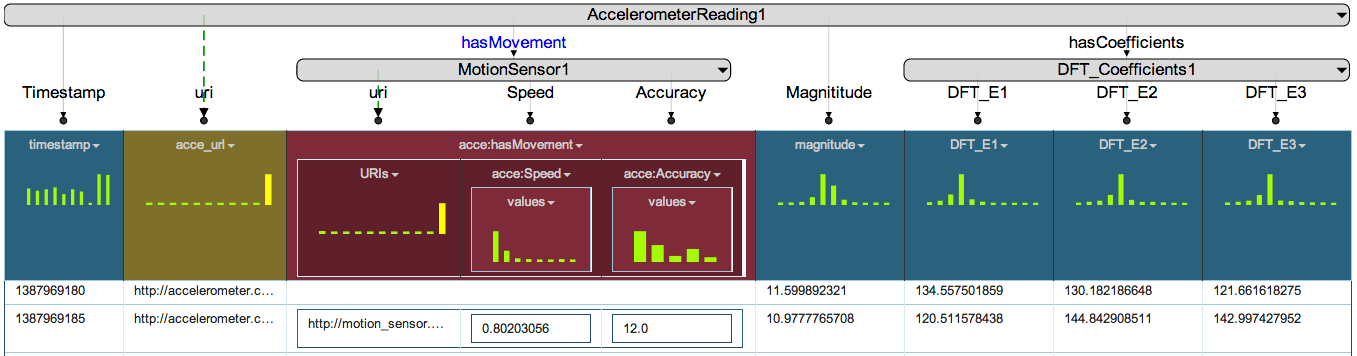
\includegraphics[width=184mm]{img/model_after_augmentation}
\caption{Karma worksheet after joining the accelerometer and location datasets}
\label{fig:model_after_augmentation}
\end{figure*}

We load the LocationProbe file, apply the `LocationProbe' model, and publish the resulting RDF. For the accelerometer sensor data, we start by loading the data collected for the first day. We apply the `AccelerometerSensorModel' and publish the RDF. To invoke the addDFT service, we select the `Invoke Service' option from the drop down menu that appears after clicking the AccelerometerReading class bubble. Karma distinguishes between service models and data models and shows the list of services that could be invoked. Karma determines that a service can be invoked if the semantic type mappings for all the input columns along with the relationships between the classes match with the model on the current worksheet. From the list of services shown, we select the addDFT service and then select the corresponding RDF graph where the accelerometer data was published. The results of the addDFT service are loaded in a new worksheet. We apply the model that was created for the addDFT output to the new worksheet and publish RDF. After we have published the data from the addDFT service, we perform a join operation with the LocationProbe data that was published previously. Starting from the topmost class in the model, i.e., AccelerometerReading, we use the `Augment Data' option to perform the join.

Karma explores the properties that could be added to the selected class, in this case the AccelerometerReading class, which are not currently present in the worksheet. Karma fetches the additional properties from the available RDF data in the triple store. In our ontology, the AccelerometerReading class has an object property `hasMovement' that connects it to the MotionSensor class. We select this property to be added in the worksheet. Karma adds a URL column for the MotionSensor class and populates it with the joined values. We repeat the join process for the MotionSensor class and add the speed and accuracy properties. The final augmented worksheet is shown in Figure \ref{fig:model_after_augmentation}. The yellow colored columns are added through transformations and the red columns are the ones that get attached by joining the location probe data. The columns in blue are part of the original model. We then publish the augmented model and the RDF in a new graph. We need to publish this model because the model shown in Figure \ref{fig:model_after_augmentation} is not the original model and contains additional properties that were added after the join operation. 

We now invoke the getLabel service to add the mode of transport column. The service creates a new worksheet to which we apply the SVM model as shown in Figure \ref{fig:svmService}, and publish the RDF. Since this is the first file that we process, we will invoke the SVM training service and use the processed data as training set. For the succeeding files, we first invoke SVM testing service and evaluate our model for the accuracy. Then we publish RDF for the test dataset to append it to the same graph that we used in the previous iteration. We use the merged data as a training set and again train our SVM model by invoking the SVM training service. We do this iteratively for the data for all the days that follow. Thus, as we process more data files, and add to the training set, our model improves in the prediction accuracy. The JSON results of the service invocation are parsed and loaded in a new worksheet. 
\section{Alternate Approach: Processing with Excel}

Microsoft Excel is one of the most widely used applications for data cleaning and preparation. It is not only easy to learn but also powerful to perform numerous computations across multiple rows and columns. Other proprietary packages that are available for data preparation are much more complex to use and usually require  user training. Despite Excel being very popular amongst users who are not tech savvy and do not possess the skills to write scripts for data preparation, we illustrate several shortcomings of using Excel for data preparation. Using Karma the user can publish models as linked data which are accessible globally for others to reuse, which is not possible using Excel files.

\begin{table}[h]
	\centering	
	\caption{Sample accelerometer data after adding magnitude\label{tab:sample_data_acce}}
  	\begin{tabular}{ | p{2cm} | p{1.3cm} | p{1cm} | p{1cm} | p{1.5cm} | }
    	\hline
	    \textbf{timestamp} & \textbf{x} & \textbf{y} & \textbf{z} & \textbf{magnitude} \\ \hline
		1387969178.5018 & 0.7374141 & 4.096479 & 10.688913 & 11.47073585 \\ \hline
		1387969180.1531 & -0.6596026 & 4.035427 & 10.85531 & 11.59989232 \\ \hline
		1387969180.1649 & -0.533907 & 4.3382936 & 10.539276 & 11.40974087 \\ \hline
		1387969180.2361 & -0.8535329 & 4.820725 & 8.850166 & 10.11401731 \\
	    \hline
  	\end{tabular}
\end{table}

One of the most important and rather annoying aspects of data preparation is its iterative nature. Users repeat the same steps to process each file in the data set. Even if the user is able to automate some parts of the data preparation using Excel, they still need to invoke the data mining services and feed in the processed files for training and testing. Moreover, using Excel does not let users share the transformations in a way that allows other users to reuse the steps recorded previously by someone. 

\begin{table}[h]
	\centering	
	\caption{Sample output after running the addDFT script\label{tab:sample_acce_dft}}
  	\begin{tabular}{ | p{1.1cm} | p{1.3cm} | p{1.4cm} | p{1.4cm} | p{1.4cm} | }
    	\hline
	    \textbf{timestamp} & \textbf{magnitude} & \textbf{DFT\_E1} & \textbf{DFT\_E2} & \textbf{DFT\_E3} \\ \hline
		1387969180 & 11.59989232 & 134.5575019 & 130.1821866 & 121.6616183 \\ \hline
		1387969185 & 10.97777657 & 120.5115784 & 144.8429085 & 142.997428 \\ \hline
		1387969214 & 11.56426981 & 133.7323362 & 140.4465978 & 150.3014305 \\ \hline
		1387969282 & 4.014597704 & 16.11699473 & 16.11699473 & 22.75025583 \\
	    \hline
  	\end{tabular}
\end{table}

We start by processing the AccelerometerSensor file for the first day. The timestamp column in the file contains decimal values; hence we change the default column format in excel, to contain decimal point upto 4 places. We then add a new column for the acceleration magnitude, that is calculated as the sum of squared values of the x,y and z coordinates. The coordinate values are fetched from their respective columns in the same file as shown in Table\ref{tab:sample_data_acce}. We apply a formula to get the magnitude value for the first row, and repeat it across the entire worksheet to calculate acceleration magnitude for the remaining rows. Once we have the magnitude, we prepare the file for DFT calculation. We select two columns --- timestamp and magnitude, and create a new file having only these columns. The addDFT Python script is executed from the command line with the newly created file as input. The script generates an output file having the DFT energy coefficients at 1Hz, 2Hz, and 3Hz of the acceleration magnitude for every 1 second time window.

The Accelerometer sensor produces a large number of readings when compared to the GPS sensor. Before using the LocationProbe file, we merge all of the files from three days into one because we only perform join operation using the LocationProbe data with the addDFT service output, and no other transformations. The accelerometer data cannot be merged because it contains continuous time-series data and the DFT calculations are performed over a time window. Merging the accelerometer data files will create gaps in the time window leading to incorrect DFT calculations. The merging of LocationProbe file is done in both our approaches. 

In the LocationProbe file, we select and copy 3 columns – `timestamp', `mSpeed', `mAccuracy' into a new worksheet. We format the timestamp column to have decimal values and add a new column, `absTimestamp', that will contain the absolute values of timestamp. We apply the `Round' formula to populate the `absTimestamp' column. In the next step, we load the output file generated from the addDFT script into a new worksheet in the current workbook. We join the two worksheets to combine the speed and accuracy columns with the DFT energy coefficients. We then add two new columns for speed and accuracy and apply the VLookUp formula to join the LocationProbe data by using the `absTimestamp' column as the key.

\begin{table}[h]
	\centering	
	\caption{Processed LocationProbe data \label{tab:processed_location_data}}
  	\begin{tabular}{ | p{2cm} | p{2cm} | p{1cm} | p{1.5cm} | }
    	\hline
	    \textbf{timestamp} & \textbf{absTimestamp} & \textbf{mSpeed} & \textbf{mAccuracy} \\ \hline
	    1387969150.56400 & 1387969151.00000 & 0 & 32 \\ \hline
 		1387969173.56800 & 1387969174.00000 & 1.3263288 & 12 \\ \hline
 		1387969185.71600 & 1387969186.00000 & 0.80203056 & 12 \\ \hline
 		1387969282.09300 & 1387969282.00000 & 1.0898862 & 24 \\
	    \hline
  	\end{tabular}
\end{table}

We add separate VLookUp formulas for each of the speed and accuracy columns to populate the respective values. For the rows that could not yield any value after the join, either for speed or for the accuracy column, we delete them and save the file as a CSV file. The missing values in the data set arise due to failure of probes --- accelerometer or GPS, while collecting data for a particular timestamp. We now execute the addLabel Python script using the previously joined file as input and generate our final processed file with the mode of transportation labels. The addLabel script attaches the mode of transportation label to each row based on the time intervals specified by the user. Table \ref{tab:sample_csv} shows the structure of the processed CSV file that is used to train and test the SVM model.

Since this is the first file that we process, we will execute the svmTraining script and use the processed data as training set. For the files from the succeeding days, we first invoke SVM testing script and evaluate our model for the accuracy. We merge the test data set with the training data set and again train our SVM model. We do this iteratively for the data from all the days to follow. Thus, as we process more data files, and add to the training set, our model improves in the prediction accuracy.

\begin{table*}[ht]
	\centering
	\caption{Structure of the processed file\label{tab:sample_csv}}
  	\begin{tabular}{ |c|c|c|c|c|c|c|c|}
    	\hline
	    \textbf{Timestamp} & \textbf{Magnitude} & \textbf{DFT\_E1} & \textbf{DFT\_E2} & \textbf{DFT\_E3} & \textbf{Speed} & \textbf{Accuracy} & \textbf{Mode} \\ \hline
	    1387869469 & 0 & 16 & 11.691308968 & 136.686705385 & 139.957767168 & 139.957767168 & walking \\ \hline
		1387870904 & 0 & 16 & 12.1850014516 & 148.474260375 & 146.964104434 & 148.759649196 & auto \\ \hline
		1387872050 & 0 & 24 & 11.3212865392 & 128.171528903 & 136.300006172 & 133.300527309 & bus \\ \hline
		1387874848 & 0 & 858 & 12.080955151 & 145.94947736 & 145.866842087 & 143.819565165 & stationary \\
	    \hline
  	\end{tabular}
\end{table*}
\section{Evaluation}
We evaluated our approach by measuring reduction in the time and effort required to perform data preparation and data mining for the mode of transport prediction task. We used a two parameter evaluation strategy (time and accuracy) to provide us with summative data to show the impact of our approach. In the following sections we discuss our experiment setup, test user's skill level and the evaluation criteria used to summarize the assessment chart. 

\subsection{Experiment Setup}
In our experiment, we evaluated the steps using Microsoft Excel and Karma for processing the entire dataset. Three sets of the AccelerometerSensor and LocationProbe dataset were collected (one set for each day).  After each step, the time required for the user to perform the task was noted along with any system processing time. For certain tasks that involved programmatic computation like calculating DFT energy coefficient values for the acceleration data, or labeling the mode of transport for individual time ranges, we used Python scripts in both the approaches. Therefore, the time taken for writing these scripts and executing them was the same in both the approaches. Hence we excluded those timings in the evaluations. We had one user to perform all the tasks in the experiment. The proficiency level of the test user was advanced, i.e., the user was thorough in using Karma and Excel. 

In order to demonstrate our objective, we asked the user to perform two trials for processing the collected data set and noted their timings. The user first prepared the collected data from day one and generated an SVM model. Then he prepared the collected data from day two and tested the day-two data with the day-one model. Finally, the user prepared the collected data from day three and tested it with the SVM model built using the data from day one and day two. When using Karma, there were one-time setup tasks in which the user first modeled all of our services by adding semantic types to the service inputs. The user modeled the following data sources and services:
\begin{enumerate}
	\item \textit{Accelerometer sensor data}: To calculate the acceleration magnitude and extract the timestamp.
	\item \textit{Accelerometer data with DFT energy coefficients} – The result of the addDFT service 
	\item \textit{LocationSensor data}: To model the speed, accuracy and timestamp columns
	\item \textit{AddDFT service}: Here we model the inputs for the addDFT service along with other meta data like service url, invocation method (GET or POST) etc.
	\item \textit{GetLabel service}: This service gets us the mode of transport for the given timestamp
	\item \textit{SVM Training}: This service model defines the SVM training and its inputs
	\item \textit{SVM Testing}: This service model defines the SVM testing and its inputs
\end{enumerate} 

Once the user had modeled all the services, he uploaded each file of the collected data and applied the semantic models. Karma automatically applied all the transformations defined in the models, so no manual effort was required. At the end of processing each file, the user invoked the SVM training and testing services. When Excel was used, the user did not need to setup the application. Table \ref{tab:excelProcessing} lists the user actions and time required to perform the task in Excel and Table \ref{tab:karmaProcessing} shows the timings when using Karma.

\subsection{Evaluation Criteria}
Our evaluation metric had two components -- efficiency and accuracy. The efficiency component included user interaction time and system processing time. The user interaction time was the time taken by the user to complete a task using the interface of the tool, for example publishing RDF in Karma or formatting column in Excel. The system processing time was the time taken by the tool to complete the computation and render the results after the user has issued the command. In terms of accuracy, we marked a data preparation task as correct if the user was able to process the data correctly and the resultant file could be used to invoke the SVM service.

\begin{table}[h]
	\centering
	\caption{Stepwise time chart for processing one file using Karma\label{tab:karmaProcessing}}
  	\begin{tabular}{ | >{\centering\arraybackslash}m{0.4cm} | >{\arraybackslash}m{3.6cm} | >{\centering\arraybackslash}m{0.6cm} | >{\centering\arraybackslash}m{1cm} | >{\centering\arraybackslash}m{0.8cm} | }
    	\hline
	    \textbf{Step} & \textbf{Task} & \textbf{User Time (sec)} & \textbf{System Processing Time (sec)} & \textbf{Total Elapsed Time} \\ \hline
	    1 & Modeling LocationProbe data & 34 & 18 & 0:52 \\ \hline
		2 & Publish RDF for LocationProbe & 12 & 6 & 1:10 \\ \hline
		3 & Modeling AccelerometerSensor data  & 18 & 5 & 1:34 \\ \hline
		4 & Publish RDF for AccelerometerSensor & 11 & 9 & 1:54 \\ \hline
		5 & Invoke addDFT service & 8 & 2 & 2:04 \\ \hline
		6 & Modeling DFT service output & 10 & 2 & 2:16 \\ \hline
		7 & Publish RDF for DFT output & 11 & 6 & 2:33 \\ \hline
		8 & Join with LocationProbe RDF & 12 & 5 & 2:50 \\ \hline
		9 & Publish the augmented model & 15 & 3 & 3:08 \\ \hline
		10 & Publish RDF for joined data & 10 & 6 & 3:24 \\ \hline
		11 & Invoke getLabel service & 8 & 2 & 3:34 \\ \hline
		12 & Filter our `NA' mode of transport & 31 & 3 & 4:08 \\ \hline
		12 & Model mode\_of\_transport data - the result of add label service & 6 & 3 & 4:17 \\ \hline
		13 & Publish RDF for Model of transport data & 20 & 4 & 4:41 \\ 
	    \hline
  	\end{tabular}
\end{table}

\subsection{Experiment Results}
Table \ref{tab:karmaProcessing} gives us the time taken for each of the data preparation tasks executed using Karma in one of the trials. The first step took the highest processing time because the combined location probe data file that was modeled, contained data from all of the three days. The transformations were executed for each step when the model was applied to this data set and since the number of rows was higher, it took more time to process. We observed that when a new worksheet is created in Karma, either by uploading a file or generated as a result of invoking a service, two steps were performed, namely applying a model and publishing the RDF. Together, these steps took roughly 20 to 25 seconds, depending upon the size of the dataset. After performing all the data transformations, RDF was published for the processed data using a new graph so that each data set can be individually used to invoke the SVM training and testing services. 

Table \ref{tab:excelProcessing} displays the time taken for the data preparation tasks executed using Excel. We can observe that the system processing time is very small when compared to Karma. This was because Excel is a native application and there is no communication latency between the interface and the application. We also observe that the user spends significant time switching between different application windows as well as the switching between the use of a mouse and keyboard. These switches were likely to introduce the most number of errors, which adds to the overall processing time. After processing the data for one day, it was stored in a new file to be used as training and testing sets for the SVM prediction task.

Table \ref{tab:timings} summarizes the timings for all of the trials. There are a number of observations that can be drawn from the table. When Karma was used, the user took the longest time to process the data set for the first day. As previously mentioned, the first iteration took more time to finish compared to the other trials since the LocationProbe data set was processed only once. However, when Excel was used, the data processing time for the first file was very close to the avarage time taken by Excel. Since most of the processing was automated in Karma, the user was relieved from repeating the commands. The time taken to invoke the SVM services for training and testing remained consistent throughout both the approaches. The Karma setup time was calculated only once as it was a one-time process. The user was also not expected to get a better result or a faster time. 

\begin{table}[h]
	\centering
	\caption{Stepwise time chart for processing one file using Excel\label{tab:excelProcessing}}
  	\begin{tabular}{ | >{\centering\arraybackslash}m{0.4cm} | >{\arraybackslash}m{3.6cm} | >{\centering\arraybackslash}m{0.6cm} | >{\centering\arraybackslash}m{1cm} | >{\centering\arraybackslash}m{0.8cm} | }
    	\hline
	    \textbf{Step} & \textbf{Task} & \textbf{User Time (sec)} & \textbf{System Processing Time (sec)} & \textbf{Total Elapsed Time} \\ \hline
	    1 & Process AccelerometerSensor data --- add magnitude and set timestamp column to be 4 decimal places & 44 & 0 & 0:44 \\ \hline
		2 & Extract timestamp and Magnitude in new worksheet and save as CSV & 41 & 0 & 1:25 \\ \hline
		3 & Invoke addDFT script & 8 & 2 & 1:35 \\ \hline
		4 & Process addDFT output file --- format timestamp column to be 4 decimal places & 12 & 0 & 1:48 \\ \hline
		5 & Copy timestamp, speed and accuracy columns from LocationProbe data into a new worksheet & 41 & 0 & 2:29 \\ \hline
		6 & Process timestamp column to be 4 decimal places, and add a new column to round off the decimal & 25 & 0 & 2:54 \\ \hline
		7 & Add vLookUp formulae in the AccelerometerData worksheet for Speed & 27 & 0 & 3:21 \\ \hline
		8 & Add vLookUp formulae in the AccelerometerData worksheet for Accuracy & 34 & 0 & 3:55 \\ \hline
		9 & Apply filter to remove unmatched --- NA rows after join and delete them. & 43 & 0 & 4:38 \\ \hline
		10 & Save this accelerometer with DFT data for input to labeling service & 19 & 0 & 4:57 \\ \hline
		11 & Invoke the labeling service over the exported CSV file  & 12 & 1 & 5:09 \\ \hline
		12 & Filter data to remove NA columns & 32 & 0 & 5:41 \\ \hline
		13 & Save the file as ProcessedData file & 6 & 0 & 5:48 \\ \hline
		14 & Copy the ProcessedData file to the required location for SVM invocation & 10 & 0 & 5:58 \\
	    \hline
  	\end{tabular}  	
\end{table}

\begin{table*}[ht!]
	\centering
	\caption{Timing summary\label{tab:timings}}
	\begin{tabular}{c|c|c|c|c|c|c|c|}
	\hline
	\multicolumn{1}{ |c }{\multirow{8}{*}{Trial 1} } &
	\multicolumn{1}{ |c| }{} & \multicolumn{3}{ c| }{Karma} & \multicolumn{3}{ c| }{Excel} \\ \cline{3-8}
	\multicolumn{1}{ |c  }{}  & \multicolumn{1}{ |c| }{} & Time & TotalSeconds & Accuracy & Time & TotalSeconds & Accuracy \\ \cline{2-8}
	\multicolumn{1}{ |c  }{}  & \multicolumn{1}{ |l| }{Dataset 1} & 4:41 min & 281 & Correct & 5:58 min & 358 & Correct     \\ \cline{2-8}
	\multicolumn{1}{ |c  }{}  & \multicolumn{1}{ |l| }{Invoke SVM training} & 0:12 min & 12 & Correct & 0:35 min & 35 & Correct   \\ \cline{2-8}
	\multicolumn{1}{ |c  }{}  & \multicolumn{1}{ |l| }{Dataset 2} & 3:20 min & 200 & Correct & 5:50 min & 350 & Correct  \\ \cline{2-8}
	\multicolumn{1}{ |c  }{}  & \multicolumn{1}{ |l| }{Invoke SVM testing on dataset2} & 0:14 min & 14 & Correct & 0:30 min & 30 & Correct \\ \cline{2-8}
	\multicolumn{1}{ |c  }{}  & \multicolumn{1}{ |l| }{Invoke SVM training using dat set 1 and 2 combined} & 0:29 min & 29 & Correct & 1:20 min & 80 & Correct \\ \cline{2-8}
	\multicolumn{1}{ |c  }{}  & \multicolumn{1}{ |l| }{Dataset 3} & 3:13 min & 193 & Correct & 5:43 min & 343 & Correct \\ \cline{2-8}
	\multicolumn{1}{ |c  }{}  & \multicolumn{1}{ |l| }{Invoke SVM testing on dataset3} & 0:12 min & 12 & Correct & 0:29 min & 29 & Correct \\ \cline{1-8}

	\multicolumn{1}{ |p{0.8cm} }{\multirow{8}{*}{Trial 2} } & \multicolumn{1}{ |l| }{Dataset 1} & 3:18 min & 198 & Correct & 5:36 min & 326 & Correct \\ \cline{2-8}
	\multicolumn{1}{ |c  }{}  & \multicolumn{1}{ |l| }{Invoke SVM training} & 0:11 min & 11 & Correct & 0:31 min & 31 & Correct   \\ \cline{2-8}
	\multicolumn{1}{ |c  }{}  & \multicolumn{1}{ |l| }{Dataset 2} & 2:49 min & 169 & Correct & 5:25 min & 325 & Correct  \\ \cline{2-8}
	\multicolumn{1}{ |c  }{}  & \multicolumn{1}{ |l| }{Invoke SVM testing on dataset2} & 0:16 min & 16 & Correct & 0:28 min & 28 & Correct \\ \cline{2-8}
	\multicolumn{1}{ |c  }{}  & \multicolumn{1}{ |l| }{Invoke SVM training using dat set 1 and 2 combined} & 0:25 min & 25 & Correct & 1:43 min & 103 & Correct \\ \cline{2-8}
	\multicolumn{1}{ |c  }{}  & \multicolumn{1}{ |l| }{Dataset 3} & 3:05 min & 185 & Correct & 5:53 min & 353 & Correct \\ \cline{2-8}
	\multicolumn{1}{ |c  }{}  & \multicolumn{1}{ |l| }{Invoke SVM testing on dataset3} & 0:14 min & 14 & Correct & 0:29 min & 29 & Correct \\ \cline{1-8}

	\multicolumn{1}{ |p{0.8cm} }{\multirow{4}{*}{Analysis} } & \multicolumn{1}{ |l| }{Total} & 22:39 min & 1359 &  & 40:20 min & 2420 &  \\ \cline{2-8}
	\multicolumn{1}{ |c  }{}  & \multicolumn{4}{ |l| }{Total Reduction excluding karma setup} & \multicolumn{2}{ l| }{17:41 min} & 42.14\%  \\ \cline{2-8}
	\multicolumn{1}{ |c  }{}  & \multicolumn{4}{ |l| }{Total Reduction including karma setup (+9:30 min)} & \multicolumn{2}{ l| }{8:11 min} & 20.28\%  \\ \cline{2-8}
	\multicolumn{1}{ |c  }{}  & \multicolumn{6}{ |l| }{Accuracy with Karma} & 100.00\%  \\ \cline{2-8}
	\multicolumn{1}{ |c  }{}  & \multicolumn{6}{ |l| }{Accuracy with Excel} & 100.00\%  \\ \cline{1-8}
	\end{tabular}	
\end{table*}

The accuracy for our experiment is the number of data preparation tasks completed correctly. We evaluated the correctness of the task as discrete Boolean values. At the end of processing a data file, if we were able to invoke the SVM training or testing service with no errors, we marked it as a successful completion. In our experiment, having 100\% accuracy at the end of all the trials for Excel and Karma does not indicate that the task is easy to perform, but it highlights the reliability and availability of using Karma to replay the transformations any number of times and always yield correct results. When using Excel, the user could  undo/redo a certain transformation to rectify any error and make sure the final result was correct it. Hence it yields 100\% accuracy while using Excel.

Both the trials showed that there was not much variation in invoking the SVM services after processing the files. The difference was in the ability to replay the steps in Karma. Every time we pick a new file to process, Karma took approximately one minute less than Excel. It took 9:30 minutes to complete the Karma setup while the execution phase took a total of 22:39 minutes to complete two trials of data preparation and mining. On the other hand, the Excel execution phase took 40:20 minutes to complete the two trials. We initially compare Karma's execution time with the total time taken for Excel since both involve repetition all of the tasks for every file. We observed a 42.14\% reduction in time taken for this iterative process by using Karma to process six data files. When we include the setup time for Karma, we observed a 20.28\% improvement in the time for the same number of files. Therefore, in our experiment, Karma requires 4 iterations of data processing to amortize the cost of its setup. 

To emphasize the potential of our results, we could extrapolate our dataset to have 100 days of mode of transportation data. Then the time spent in preparing the data using Excel could be approximately 670 minutes. However the process could be completed in approximately 387 minutes using Karma, which also included the setup time. When we processed 6 files, Karma's setup time caused the time reduction to decrease from 42.14\% to 20.28\%. But when we processed 100 files, the reduction ratio is more or less the same even if the Karma setup time is included or excluded. 

We also discuss another important scenario where multiple users of the same skill level are involved in our experiment to process the data. For example, we will consider 10 users participating in our experiment. If every user is using Karma individually, they will all roughly need 9:30 minutes to setup Karma and 22:39 minutes to process the files. A total of 5.3 person hours is spent in data preparation. Here the real benefit of modeling data source and services to an ontology using Karma, is the ability to share models across users. Therefore, if one user spent his 9:30 minutes in setting up Karma and shares the models with all the other users, the data preparation task is completed in 3.7 hours, saving 26\% of the time that was required previously. Based on the observations, we can conclude that Karma improves efficiency in data preparation and data mining on large data sets by reducing time taken and manual efforts.
\section{Related Work}

Preparing raw data for a data mining task typically reqiures mulitple data transformation steps. Many of these tasks are common across a large number of data mining applications, such as dealing with missing values, discretization, and normalization. However, in many cases, these are not sufficient and other transformation steps are required which are specific to the problem being solved.

Popular data mining software suites like RapidMiner\footnote{http://rapidminer.com/products/rapidminer-studio} and KNIME\footnote{http://www.knime.org/knime} allow most of the common transformation steps. However, when it comes to performing data transformation tasks that are specific to the problem at hand, a majority of these suites do not provide support for such specialized transformations.

There are also data preparation tools like DataPreparator\footnote{http://www.datapreparator.com} that offer most of the common data transformation tasks and operations like merging data from different files to prepare the data for mining, but these tools are just for data preparation and mining has to be done separately, unlike our end-to-end approach. Moreover, these tools do not provide support for problem-specific custom data transformation tasks.

Google Refine\footnote{https://code.google.com/p/google-refine/} is another data transformation tool which has data cleaning capabilities, and supports some commonly used data transformation tasks. It also supports custom text transformations to modify text in data cells. Like in the case of other data preparation tools, data mining has to be done separately as Google Refine does not have data mining capabilities.

Our work provides an end-to-end integrated approach for data preparation and mining, with support for problem-specific transformation tasks as features, extensions, or services. More- over, our work allows automation of data preparation tasks, which reduces the time taken to prepare data for mining.
\section{Discussion}
This paper presented a unified approach to data preparation and mining using the data integration system, Karma. We discussed an end-to-end approach of data preparation and data mining, which consists of various transformations applied on a data set, publishing the data as RDFs, joining different data sets based on their mapping to the ontology, modeling the data mining services to a domain model, and invoking theses services with the published data. Our work on Karma provided us with a platform to record the various transformations that the user performs in preparing the raw data set to its desired form. We achieved a significant improvement in reducing the time taken for this iterative process of data preparation by replaying the transformations the user performed on the first file, on all the other files in our data set. We also showed how services could be modeled using semantics and reused by publishing them as linked data.

% conference papers do not normally have an appendix


% use section* for acknowledgement
%\section*{Acknowledgment}


%The authors would like to thank...





% trigger a \newpage just before the given reference
% number - used to balance the columns on the last page
% adjust value as needed - may need to be readjusted if
% the document is modified later
%\IEEEtriggeratref{8}
% The "triggered" command can be changed if desired:
%\IEEEtriggercmd{\enlargethispage{-5in}}

% references section

% can use a bibliography generated by BibTeX as a .bbl file
% BibTeX documentation can be easily obtained at:
% http://www.ctan.org/tex-archive/biblio/bibtex/contrib/doc/
% The IEEEtran BibTeX style support page is at:
% http://www.michaelshell.org/tex/ieeetran/bibtex/
% argument is your BibTeX string definitions and bibliography database(s)
%\bibliography{IEEEabrv,../bib/paper}
%
% <OR> manually copy in the resultant .bbl file
% set second argument of \begin to the number of references
% (used to reserve space for the reference number labels box)

\bibliographystyle{IEEEtran}

%%%%%% Uncomment bibliography below after adding references to bibliog.bib
\bibliography{bibliog}

\end{document}


